%%%%%%%%%%%%%%%%%%%%%%%%%%%%%%%%%%%%%%%%%
% Beamer Presentation
% LaTeX Template
% Version 1.0 (10/11/12)
%
% This template has been downloaded from:
% http://www.LaTeXTemplates.com
%
% License:
% CC BY-NC-SA 3.0 (http://creativecommons.org/licenses/by-nc-sa/3.0/)
%
%%%%%%%%%%%%%%%%%%%%%%%%%%%%%%%%%%%%%%%%%

%----------------------------------------------------------------------------------------
%	PACKAGES AND THEMES
%----------------------------------------------------------------------------------------

\documentclass{beamer}

\mode<presentation> {

% The Beamer class comes with a number of default slide themes
% which change the colors and layouts of slides. Below this is a list
% of all the themes, uncomment each in turn to see what they look like.

%\usetheme{default}
\usetheme{AnnArbor}
%\usetheme{Antibes}
%\usetheme{Bergen}
%\usetheme{Berkeley}
%\usetheme{Berlin}
%\usetheme{Boadilla}
%\usetheme{CambridgeUS}
%\usetheme{Copenhagen}
%\usetheme{Darmstadt}
%\usetheme{Dresden}
%\usetheme{Frankfurt}
%\usetheme{Goettingen}
%\usetheme{Hannover}
%\usetheme{Ilmenau}
%\usetheme{JuanLesPins}
%\usetheme{Luebeck}
%\usetheme{Madrid}
%\usetheme{Malmoe}
%\usetheme{Marburg}
%\usetheme{Montpellier}
%\usetheme{PaloAlto}
%\usetheme{Pittsburgh}
%\usetheme{Rochester}
%\usetheme{Singapore}
%\usetheme{Szeged}
%\usetheme{Warsaw}

% As well as themes, the Beamer class has a number of color themes
% for any slide theme. Uncomment each of these in turn to see how it
% changes the colors of your current slide theme.

%\usecolortheme{albatross}
\usecolortheme{beaver}
%\usecolortheme{beetle}
%\usecolortheme{crane}
%\usecolortheme{dolphin}
%\usecolortheme{dove}
%\usecolortheme{fly}
%\usecolortheme{lily}
%\usecolortheme{orchid}
%\usecolortheme{rose}
%\usecolortheme{seagull}
%\usecolortheme{seahorse}
%\usecolortheme{whale}
%\usecolortheme{wolverine}

%\setbeamertemplate{footline} % To remove the footer line in all slides uncomment this line
%\setbeamertemplate{footline}[page number] % To replace the footer line in all slides with a simple slide count uncomment this line

%\setbeamertemplate{navigation symbols}{} % To remove the navigation symbols from the bottom of all slides uncomment this line
}

\usepackage{graphicx} % Allows including images
\usepackage{booktabs} % Allows the use of \toprule, \midrule and \bottomrule in tables
%\usepackage{movie15}
%%%%% SPECIAL PACKAGES %%%%%%%%%%
\usepackage{setspace}
%\usepackage[ngerman]{babel}
\usepackage[utf8]{inputenc}
\usepackage{fancyhdr}
\usepackage{tabularx}
%\renewcommand{\rmdefault}{phv}
%\renewcommand{\sfdefault}{phv}

\setcounter{tocdepth}{2} % to get subsubsections in toc 
% cf. http://www.latex-community.org/forum/viewtopic.php?f=47&p=44760

\usepackage{amssymb,latexsym}
\usepackage{amsmath, amsthm}
\usepackage{mathabx}

%for bibliography; installation using 'sudo tlmgr install amsrefs'
\usepackage{amsrefs}

\usepackage{graphics}
\usepackage{animate}
%\usepackage{xmpmulti}

\usepackage{hyperref}
\hypersetup{colorlinks=true, urlcolor=blue}

\usepackage{cancel} % http://jansoehlke.com/2010/06/strikethrough-in-latex/

\usepackage{listings} % http://en.wikibooks.org/wiki/LaTeX/Source_Code_Listings
% http://olmjo.com/files/teaching/PSC505/LaTeXandR.pdf

% package for flower symbol (\ding(96))
\usepackage{pifont}
% required installation: sudo apt-get install texlive-fonts-recommended (30MB)
% http://tug.ctan.org/info/symbols/comprehensive/symbols-a4.pdf

\usepackage{tikz} % for diagrams
\usetikzlibrary{matrix,positioning,arrows,calc,decorations.pathmorphing,shapes}
% for snaky lines (http://tex.stackexchange.com/questions/209942/curved-arrows-in-tikz) 
\tikzset{snake it/.style={-stealth,
decoration={snake, 
    amplitude = .4mm,
    segment length = 2mm,
    post length=0.9mm},decorate}}

\usepackage[parfill]{parskip}

\usepackage{framed} %for putting some text in boxes using \begin{framed}

\usepackage{enumerate}

%for displaying tensor indices properly. requires installation of tensor package using 'sudo tlmgr install tensor'
\usepackage{tensor}

%for placing captions of figures on the side instead of above/below the figure
\usepackage{sidecap}
\linespread{1.2}

%plain makes sure that we have page numbers
%\pagestyle{plain}

\theoremstyle{plain}
\newtheorem{axiom}{Axiom}
\newtheorem*{main}{Main Theorem}
\newtheorem{proposition}{Proposition}

\theoremstyle{definition}

\theoremstyle{remark}
\newtheorem*{notation}{Notation}

\numberwithin{equation}{section}
\numberwithin{figure}{section}
\numberwithin{theorem}{section}
\usepackage{bibentry}

%symbol for maps
\renewcommand{\to}{\longrightarrow}
\newcommand{\injmapto}{\hookrightarrow}
\newcommand{\surjmapto}{\twoheadrightarrow}
\newcommand{\linearmapto}{\stackrel{\sim}{\longrightarrow}}
\newcommand{\projmapto}{\stackrel{\pi}{\longrightarrow}}

%for real numbers
\newcommand{\R}{\mathbb{R}}

% manifold, atlas and topology
\newcommand{\A}{\mathcal{A}}
%\newcommand{\O}{\mathcal{O}}
\newcommand{\mfd}{(M, \mathcal{O}, \mathcal{A})}

\newcommand{\after}{\circ}
\newcommand{\stdtop}{\mathcal{O}_{std}}
\newcommand{\cibasis}[2][]{\frac{\partial #1}{\partial #2}}

%connection coefficient functions or gammas
\newcommand{\ccf}[2]{\Gamma\indices{^{#1}_{#2}}}
\newcommand{\ccfx}[3]{\left(\Gamma_{#3}\right)\indices{^{#1}_{#2}}} % with chart index

%set theory symbols
%\renewcommand{\exists}{\exists\,}
%\renewcommand{\forall}{\forall\,}

%This defines a new command \questionhead which takes one argument and prints out Question #. with some space.
\newcommand{\questionhead}[1]
  {
   \noindent{\small\bf Question #1.}
  }

\newcommand{\problemhead}[1]
  {
   \noindent{\small\bf Problem #1.}
  }

\newcommand{\exercisehead}[1]
  { \smallskip
   \noindent{\small\bf Exercise #1.}
  }

\newcommand{\solutionhead}[1]
  {
   \noindent{\small\bf Solution #1.}
  }

\newcommand{\bubblethis}[2]{
  \tikz[remember picture,baseline]{\node[anchor=base,inner sep=0,outer sep=0](#1) {#1};\node[overlay,cloud callout,callout relative pointer={(0.2cm,-0.7cm)}, aspect=2.5,fill=white!90] at ($(#1.north)+(-0.5cm,1.6cm)$) {#2};}
}



%%%%%%%%%%%%%%%%%%%%%%%%%%%%%


%----------------------------------------------------------------------------------------
%	TITLE PAGE
%----------------------------------------------------------------------------------------
\title[LLM Survey]{LLM Survey} % The short title appears at the bottom of every slide, the full title is only on the title page

\author{Piyush Kaul } % Your name
\institute[https://piyushkaul.github.io] % Your institution as it will appear on the bottom of every slide, may be shorthand to save space
{
 \\ % Your institution for the title page
\medskip
\textit{piyushkaul@ieee.org} % Your email address
}
\date{\today} % Date, can be changed to a custom date

\begin{document}

\begin{frame}
\titlepage % Print the title page as the first slide
\end{frame}

\begin{frame}
\frametitle{Overview} % Table of contents slide, comment this block out to remove it
\tableofcontents % Throughout your presentation, if you choose to use \section{} and \subsection{} commands, these will automatically be printed on this slide as an overview of your presentation
\end{frame}

%----------------------------------------------------------------------------------------
%	PRESENTATION SLIDES
%----------------------------------------------------------------------------------------

%------------------------------------------------
\section{LoRA} % Sections can be created in order to organize your presentation into discrete blocks, all sections and subsections are automatically printed in the table of contents as an overview of the talk
%------------------------------------------------


\begin{frame}
\frametitle{LoRA - Low Rank Adaptation of LLM}
Objective
\begin{enumerate}
  \item The trained LLMs are generic. Need to be fined tuned for tasks. 
  \item Not possible to train LLM without enormous amout of GPUS/Compute power.
  \item Weight changes due to fine tuning can be modelled as Low Rank layers in parallel.
  \item We only allow the added Low Rank Dcomposition layers to tain.
  \item For GPT3, 175 MB, low rank of 2 is adequate. Full rank being quite large.
\end{enumerate}
\end{frame}

\begin{frame}[shrink]
\frametitle{LoRA - Low Rank Adaptation of LLM}
For pre-trained matrix $W_0$, the augmented networks is defined as.
\begin{align}
    W_0 + \delta W = W_0 + BA
\end{align}
where $B \in R^{d \times r}$ and $A\in R^{r\times k}$
\begin{enumerate}
\item $W_0$ stays frozen whereas only B and A are trained
\item The basic model weight set $W_0$ is common across tasks and only B and A need to be switched.
\item Generalization is possible for full fine-tuning as well.
\item Only the attention weights need to be fine tuned. The MLP weight can stay frozen.
\end{enumerate}
\end{frame}

\begin{frame}
\frametitle{LoRA - Results}
\begin{enumerate}
    \item Reduce memory size by 1000 times. 350 GB $\to$ 35 MB
\end{enumerate}
\end{frame}


\begin{frame}
\frametitle{LoRA - Layer Decomposition}
\begin{figure}
    \centering
    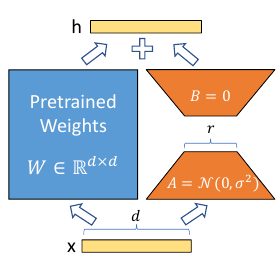
\includegraphics[width=0.5\linewidth]{lora.png}
    \caption{Enter Caption}
    \label{fig:enter-label}
\end{figure}
\end{frame}


                        
\section{QLoRA}
\begin{frame}
\frametitle{QLoRA: Efficient Fine-tuning of Quantized LLM}
QLoRA reduces memory requirement from $>$ 700 GB of GPU to $<$48 GB
Following advantages are mentioned
\begin{enumerate}
    \item 4-bit Normal Float. Better than 4-bit integer and 4-bit float
    \item Double Quantization. Quantizing Quant info (saving of approx 3GB for 65 GB)
    \item Paged Optimizers. Avoid gradient check pointing spikes.
\end{enumerate}
\end{frame}

\begin{frame}[shrink]
    \frametitle{QLoRA: 4-bit Normal Float}
    \begin{enumerate}
        \item Storage as 4b NF. Convert to BF16 for usage.
        \item The main limitation of quantile quantization is estimating quantiles.
        \item We fix the datatype range [-1,1]. The quantiles of datatype and NN weights need to be matched
        \item Estimate $2^{k+1}$ quantiles for $N(0,1)$ to obtain k-bit quantile regression
        \item Normalize its values in [-1, 1] range
        \item Quantize input by Re scaling to [-1,1] range
    \end{enumerate}                        

    \begin{align}
        q_i = \frac{1}{2} (Qx(\frac{i}{2^k+1}) + Qx(\frac{i+1}{2^k+1})    
    \end{align}
    To solve the problem or representing zero exactly, we do this separately for +ve and -ve range.
\end{frame}                        


\section{ZeroQuant-FP}
\begin{frame}
\frametitle{ZeroQuant-FP}
Contribution
\begin{enumerate}
    \item Negligible degradation from FP16 to FP8
    \item FP8 activation along with FP4 weights. LoRC compensates quantization error for w4a8
    \item FP4 weights need to be converted to FP8 for inference. Can be done dynamically. 
    \item Complexity reduction by having scale factors only in power of 2
\end{enumerate}
\end{frame}

\begin{frame}
\begin{figure}
    \centering
    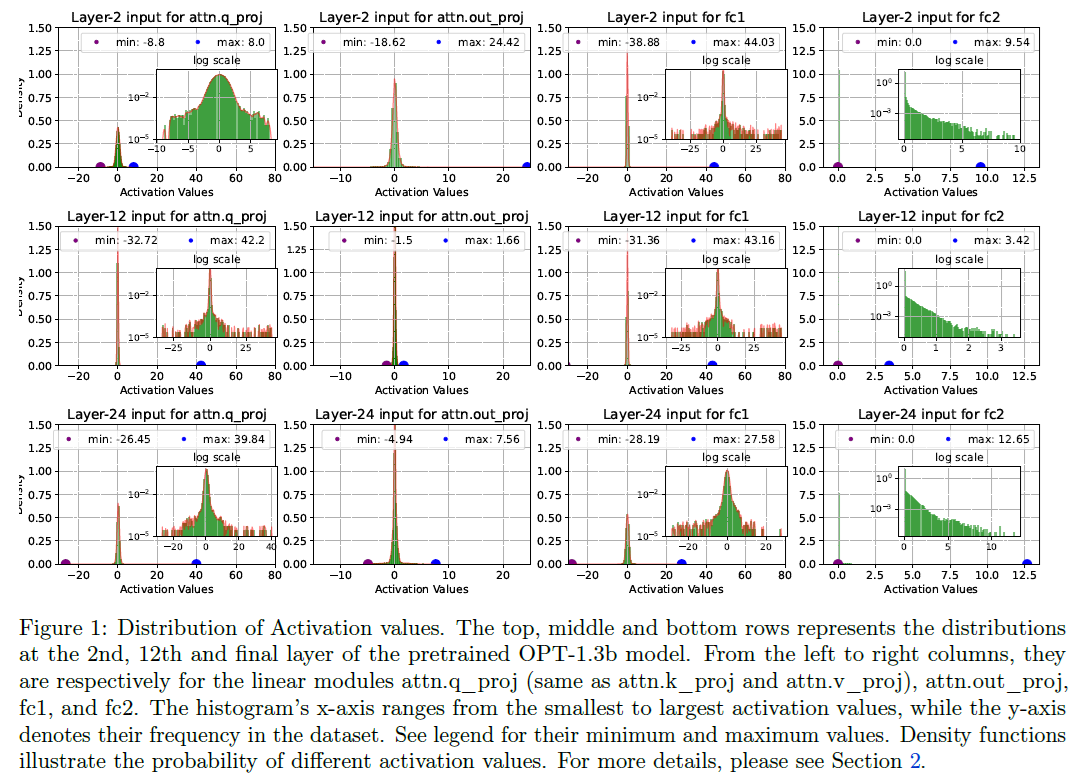
\includegraphics[width=0.9\linewidth]{distribution.png}
    \caption{Distribution of Activation Values}
    \label{fig:distribution-of-activation}
\end{figure}
\end{frame}


\begin{frame}
\frametitle{ZeroQuant-FP - Observations}
\begin{enumerate}
    \item Input to q-proj is Normal
    \item The output of q-proj and FC are skewed
    \item Integer quantization is not ideal to process skewness
    \begin{align}
        Q(x) = INT(X- Z/S) - Z
    \end{align}
    \item Integer quantization not ideal for outliers.
\end{enumerate}
\end{frame}

\begin{frame}
\frametitle{INT8 vs FP8}
\begin{figure}
    \centering
    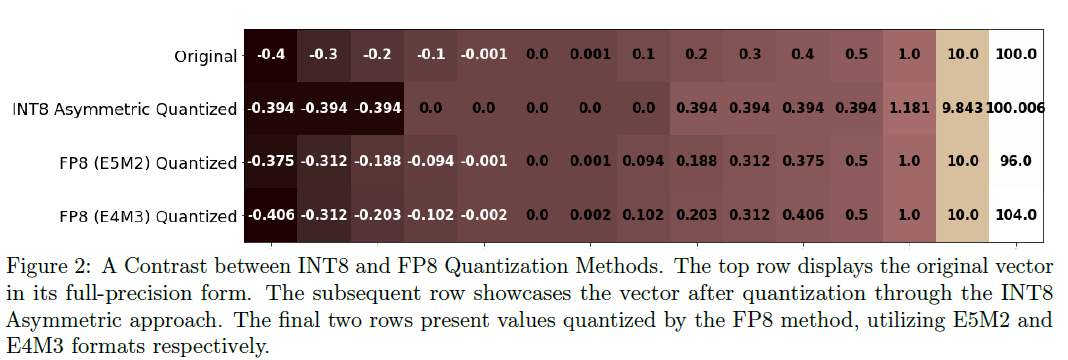
\includegraphics[width=1\linewidth]{int8_vs_fp8.png}
    \label{fig:in8_vs_fp8}
\end{figure}
\end{frame}

\begin{frame}
\frametitle{Techniques Used}
\begin{enumerate}
    \item Zero Quant V2 (FGQ and Token Wise Quantization)
    \item LoRC
    \item Casting FP8 to FP4 with restricted scale
\end{enumerate}
Two methods used for restricting the scale
\begin{enumerate}
    \item Map to nearest values represented by power of t2 i.e. $\hat{S} = 2^{log_2(S)}$
    \item Collect scale in vector $s= [S_1,.. S_x]$. Take maximum and denote by $S_{max}$. Adjust  $S_{max}/s$
\end{enumerate}
\end{frame}




\begin{frame}{Zero Quant FP}
    To be represented by power of 2. Then define
    \begin{align}
    \hat{S_i} = S_{max}/2^{ [log_2(S_{max}/S_i)]}    
    \end{align}
\end{frame}

\begin{frame}
\frametitle{Results}
\begin{figure}
    \centering
    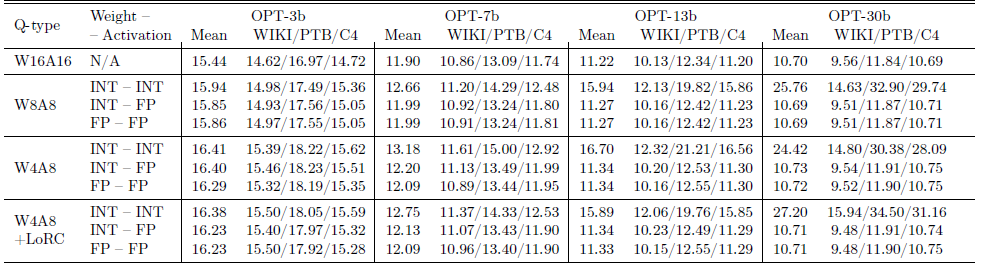
\includegraphics[width=0.9\linewidth]{results_int8_vs_fp4.png}
    \caption{Results}
    \label{fig:int4_vs_fp4_results}
\end{figure}
\end{frame}
\section{Zero Quant V2}


%\begin{frame}
%\frametitle {Zero Quant V2: Sensitivity Analysis}
%\begin{enumerate}
%\item INT8 weight-only quantization can serve as a standard
%method for reducing memory costs in LLMs, with negligible degradation in accuracy.
%\item INT4
%weight-only quantization for small models results in substantial accuracy degradation (Class-3), but
%this effect lessens as the model size increases (Class-2)
%\item Contrary to (2), INT8 activation results in
%minimal accuracy drops for small models (Class-1) but larger models exhibit greater drops (Class-3).
%\item  With INT8 activation, BLOOM shows no divergence issues up to a model size of 176B, whereas
%OPT performs poorly from ≥ 6.7B model sizes.
%\end{enumerate}
%\end{frame}

\begin{frame}[shrink]
Following Algorithms were tried.
\begin{enumerate}
    \item RTN
    \item GPTQ
    \item ZQ-Global
    \item ZQ-Local
\end{enumerate}
Following results were obtained
\begin{enumerate}
    \item GPTQ typically performs better for weight-only quantization, while
ZeroQuant (including both ZQ-Global and ZQ-Local
) yields superior results for weight and activation
quantization. 
    \item The tested optimization-based methods cannot achieve Class-1 quantization error
for either INT4 weight-only or W4A8 quantization with the exception of GPTQ on OPT-30B with
weight-only quantization.
\end{enumerate}
\end{frame}
\section{Outlier Suppression}

\begin{frame}{Outlier Suppression}
\begin{enumerate}
    \item Channel Wise Shifting and  Scaling
    \begin{align}
        \Tilde{X} = (X - Z) \bigodiv s
    \end{align}
    \item Unified migration pattern
    \begin{align}
    \Tilde(X) \bigodiv s) W^T + zW^T + b = (\Tilde{X} \bigodiv s ) W^T + zW^T + b \\
    = \Tilde{X} (w^T \bigodiv s^T) + (zW^T + b)
    \end{align}
\end{enumerate}
\end{frame}

\begin{frame}{Joint Optimization}
Joint Optimization of weights and activations is done by minimizing quantization loss
Activation loss is given by
\begin{align}
    min_s[[||Q((X-Z]\bigodiv s) - (X-Z) \bigodiv s||^2_F]
\end{align}  
\end{frame}
\section{Optimal Brain Surgeon}
\begin{frame}
\frametitle{Optimal Brain Surgeon}
\begin{enumerate}
    \item OBS permits a 90\%, a 76\%, and a 62\% reduction in weights over back-propagation with weight decay on three benchmark Monk's problems 
    \item Of OBS, Optimal Brain Damage, and magnitude-based methods, only OBS deletes the correct weights from a trained XOR network in every case. 
    \item Optimal Brain Surgeon makes no restrictive assumptions about the form of the network's Hessian, and thereby eliminates the correct weights. 
    \item OBS does not demand (typically slow) retraining after the pruning of a weight
\end{enumerate}
\end{frame}
\begin{frame}[shrink]
\frametitle{Optimal Brain Surgeon}
Taylor series of error with respect to weights is 
\begin{align}
    \delta E = \left(\frac{\partial E }{\partial \mathbf{w}}\right) \cdot \delta\mathbf{w} + \frac{1}{2} \delta \mathbf{w}^T \cdot \mathbf{H} \cdot \delta w + O(|| \delta \mathbf{w} ||^3)
\end{align}
With training convergence, 1st term is assumed zero. Third term is also ignored.
For pruning we express
\begin{align}
    e^T_q \cdot \delta w  + w_q = 0
\end{align}
Using the above two We form the Lagrangian
\begin{align}
\frac{1}{2} \delta w^T \cdot H \cdot \delta w + \lambda (e^T_q \cdot \delta w + w_q)
\end{align}

\end{frame}
\begin{frame}{Optimal Brain Surgeon}
We solve the above Lagrangian to arrive at the optimal weight change
\begin{align}
    \delta w = \frac{w_q}{[\mathbf{H}^{-1}_{qq}]}\mathbf{H}^{-1} e_q
\end{align}
and corresponding change in loss
\begin{align}
\delta L_q = \frac{1}{2} \frac{W_q^2}{H^{-1}_{qq}}
\end{align}
\end{frame}
\begin{frame}{Optimum Brain Surgeon}
\begin{enumerate}
    \item Train a "reasonably large" network to minimum error.
    \item Compute $H^{-1}$ .
    \item Find the q that gives the smallest saliency $L_q = W_q^2/(2[H^{-1}]_{qq})$. If this candidate error
            increase is much smaller than E, then the qth weight should be deleted, and we
            proceed to step 4; otherwise go to step 5. (Other stopping criteria can be used too.)
    \item Use the q from step 3 to update all weights (Eq. 5). Go to step 2.
    \item No more weights can be deleted without large increase in E. (At this point it may be
desirable to retrain the network.
\end{enumerate}
\end{frame}
\begin{frame}
\begin{figure}
    \centering
    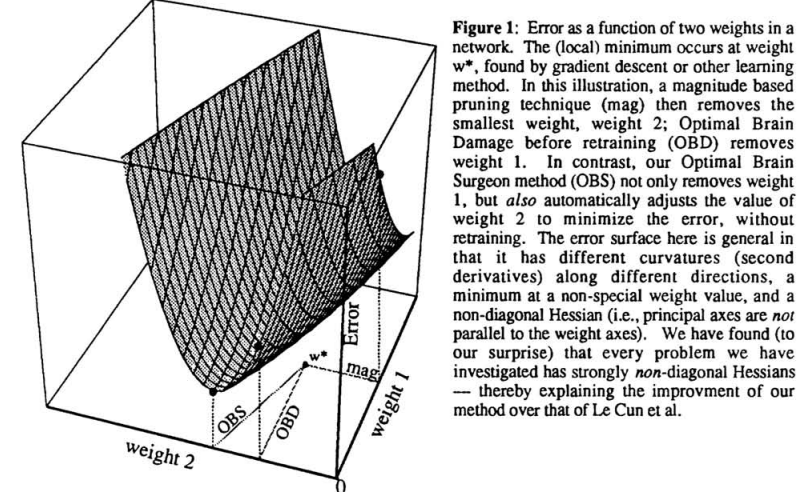
\includegraphics[width=0.9\linewidth]{obs.png}
    \caption{Enter Caption}
    \label{fig:enter-label}
\end{figure}
\end{frame}
\section{Optimal Brain Compression}
\section{GPTQ}


%------------------------------------------------

\begin{frame}[t, allowframebreaks]
\frametitle{References}
%\bibliographystyle{amsalpha}
%\bibliography{references}
\end{frame}

%------------------------------------------------

\begin{frame}
\Huge{\centerline{The End}}
\end{frame}

%----------------------------------------------------------------------------------------

\end{document} 